\chapter{Monte Carlo シミュレーションにおける実験評価}\label{simulation}

この章では,実験が適切に構築されていることをMonte Carloシミュレーションを用いて評価する.
また,期待されるスペクトルを推定する.

\section{Monte Carlo シミュレーションの意義}

本実験では,複雑に物体が組み合わされており,我々が求めるイベントがどれくらいの頻度で発生しうるのかを計算するのは立体角や断面積の計算が入り組みかなり難しい.
そこでMonte Carloシミュレーションを用いて,実験レートを評価する.本実験では,Monte CarloシミュレーションとしてGeant4\cite{geant4}を用いてプラスチックシンチレータの中で停止せずに陽電子がターゲットに到達するか,そしてターゲットから発生したガンマ線がNaIシンチレータでエネルギーを落とすかを確かめた.
また,実験でのバックグラウンドを推定した.

今回用いた線源は$\ce{^{22}Na}$ の標準線源であり,200 kBqのものである.
この線源強度と我々の実験期間約1週間を考慮して,1 Hzの実験レートとS/N比100を目標に実験のデザインが適当か検証した.

線源の$\beta$崩壊から考えると実験の各過程はごく稀なイベントであり,一度に全てのジオメトリを実装して実験を行うのは効率が悪い.
今回は本実験でオルソポジトロニウムの寿命を測定する過程の評価を,$\ce{^{22}Na}$ 線源が$\beta$ 崩壊した陽電子がシンチレーターを通過してシリカゲルに到達する過程のレート評価,線源から直接NaIシンチレータに入る$\gamma$ 線の評価,そして形成されたポジトロニウムが崩壊し,放出された$\gamma$ 線がNaIシンチレータで落とすエネルギーの評価の3つに分割してシミュレーションを行った.
これらを統合して考える事で効率よく適切な評価を行うことができる.
プログラムの実装の都合上,シミュレーション結果に関係の無い\ce{^{22}Na}の寿命のみ,付属のライブラリを書き換えた.

\section{プラスチックシンチレーターの通過}
\label{section_test1}

\subsection{概要}
今回の実験で用いられたプラスチックシンチレータは0.15 mmの厚みのものである.線源から放出される陽電子が,シンチレータ内で停止してしまうとシリカゲルに到達せずポジトロニウムを形成することができない.
ポジトロニウムを形成するためには,陽電子がまず標準線源の0.1mmの厚みのアルミ窓を通過して,空気中を伝播し,さらにシンチレータをエネルギーを落としきること無く通過する必要がある.
実際の線源を忠実に再現したジオメトリを作成し,シンチレータと線源の距離を変えながら通過してくる粒子の割合を調べた.

このとき,ポジトロニウムのミキシングを起こすために用いる磁場0.1Tは,陽電子をシリカゲルまで導く方向になるよう設定した.実際の実験でもこの方向に磁場を使用することが可能である.

\subsection{ジオメトリ}

\begin{figure}[htbp]
	\centering
		\includegraphics[width=10cm]{img/test1_geometry.pdf}
	\caption{構築したジオメトリ}
	\label{test1_geometry}
\end{figure}

図\ref{test1_geometry} はプラスチックシンチレーターの試験として作成したジオメトリで,標準線源とその表面から距離$d$ mm離れたターゲットである$\phi8$ mm,厚み0.15 mmのプラスチックシンチレーター(赤),その直後に置かれた理想的な粒子検出器で構成されている.
非常に多くの緑の線で示されているのが$\gamma$線,青の線で示されているのが陽電子の軌跡である.図ではイベント例として\ce{^{22}Na}が100個崩壊した軌跡を表示している.
標準線源はデータシートにしたがって作成し,アクリルのケースと0.1 mm厚のアルミニウム製の窓を実装してある.理想的な粒子検出器は入射した粒子の種類とエネルギーが分解能無限大で確実にわかる.
\ce{^{22}Na}はbranching ratioにしたがって$\beta^+$崩壊する.

\subsection{陽電子到達数と立体角}

プラスチックシンチレーターを線源から遠くに置くほど,透過する陽電子数は減少すると考えられる.この減少には,空気中を伝播する際に陽電子が相互作用することも影響すると考えられるが,大部分の影響は立体角の減少に由来すると予想される.今回は理想的な粒子検出器を実装しているため,ニュートリノの数を調べることでも立体角を概算する事ができる.無論,立体角$\Omega$ srを解析的に計算することも可能で,

\begin{equation}
	\Omega = 2\pi \left( 1-\cos\left(\arctan\frac{8.0/2}{d+2.5}\right)\right)
\end{equation}

で与えられる.今回は$d$を線源の表面からシンチレーターを通過するまでの距離と定義しているので,放射線源中心からの補正2.5 mmを加えている.

\subsection{磁場の援用}
概要でも触れたが,ポジトロニウムのミキシングを起こさせるための磁場を,陽電子をターゲットまで導くことにも援用することができる.
強力に磁場方向に引き寄せられるのが見て取れるので,磁場をかけたとき,かけないときで実験レートを比較する.

\subsection{結果}

図\ref{test1}は$d=100$mmで,100Mイベント生成した際のシンチレーターを通過した陽電子のエネルギースペクトル(青)である. シンチレーターを外したとき(赤)と比較した.

また,図\ref{scinti_test}がシンチレーターを陽電子が通過する割合の距離依存である.磁場をかけたとき(赤)と磁場をかけていないとき(青)をプロットし,計算された立体角に定数を乗じて$d=10$mmの磁場なしの点と重なるようにプロットした.

\begin{figure}[htbp]
	\centering
		\includegraphics[width=10cm]{fig/test1.pdf}
	\caption{シンチレータを透過した陽電子のエネルギー}
	\label{test1}
\end{figure}


\begin{figure}[htbp]
	\centering
		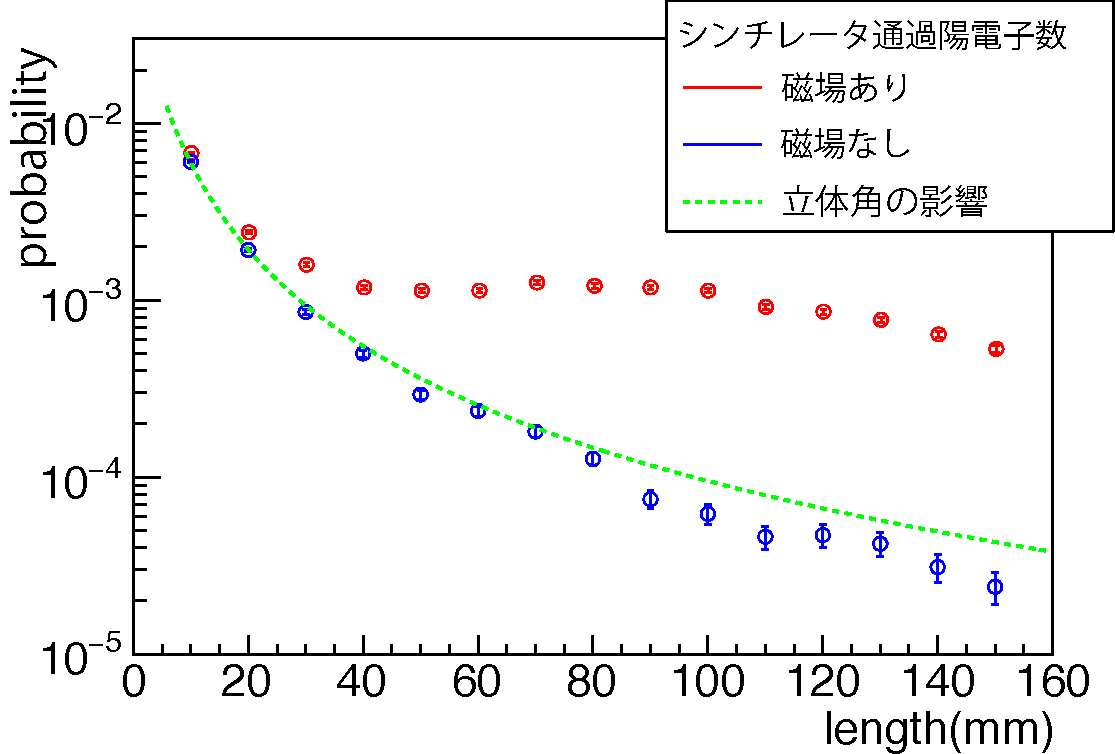
\includegraphics[width=10cm]{fig/scinti_test.pdf}
	\caption{プラスチックシンチレータ通過粒子割合}
	\label{scinti_test}
\end{figure}

\subsection{考察}

結果\ref{test1}では,シンチレータを通過してきた陽電子のエネルギースペクトルを再現している.プラスチックシンチレータでおよそ40\%程度陽電子を損失するが,約1/1000の陽電子が到達し実験に十分な陽電子が通過していると判断する.

一方で,磁場をかけたときとかけていないときで,陽電子の到達数には差がある,
磁場の無いときは陽電子数は距離が伸びるにつれてほぼ立体角に従い減り続けていくが,磁場のある際には40-110 mm程度まで陽電子数に大きな変化がない.この結果より実際の設計ではターゲットであるシリカゲルまで100 mm程度線源から離した.線源から出る$\gamma$線が直接NaI(Tl)シンチレータに入らないように遮蔽することを考えるとシンチレータの極近くに線源を置くことは現実的ではないため,できる限り離れつつもレートを確保することをねらったためである.

\subsection{鉛コリメータの実装}
実験の可視化より,バックグラウンドが非常に多くなる事が予想されるため,鉛のコリメータを置くことを考えた.

\begin{figure}[htbp]
	\centering
		\includegraphics[width=10cm]{img/test1b_geometry.pdf}
	\caption{実装した鉛コリメータ}
	\label{test1b_geometry}
\end{figure}

\begin{figure}[htbp]
	\centering
		\includegraphics[width=10cm]{fig/collimator_loss.pdf}
	\caption{鉛コリメータで失われる陽電子}
	\label{collimator_loss}
\end{figure}

図\ref{test1_geometry}は鉛のコリメータを実装した様子である.先の考察から線源までの距離を100 mmとし,そこに鉛のコリメータをおいた.NaIシンチレータをできる限りターゲットに近づけて立体角を大きくすることを考えるため,鉛のコリメータは72 mmの幅,高さと奥行きを100 mmで設計した.また,$\phi16$の穴をターゲットに向けて空けた.ターゲット側では$\gamma$線が大きく落とされている.

図\ref{collimator_loss}は鉛のコリメータをおいたとき(赤)と置かないとき(青)の到達する陽電子数の比較である.大きなバックグラウンドの減少を狙ったがそれだけでなく,イベント数も鉛コリメータの壁面に陽電子が衝突してしまうことで減少すると考えられる.

このイベント数の減少に対するバックグラウンド事象数の減少は,第\ref{section_test2}節で評価する.

\section{線源からのバックグラウンド評価}
\label{section_test2}

\subsection{概要}
第\ref{section_test1}節で,プラスチックシンチレータの評価で,ターゲットであるシリカゲルに到達する陽電子数について定量的に見積もることができた.
次に我々の求めている事象に対して,バックグラウンドとなる線源から直接出る$\gamma$線がどのくらい多いのかを評価する.


\subsection{ジオメトリ}
実際の実験装置とほとんど同じジオメトリを構築し,シミュレーションを行った.図\ref{test2_geometry}が構築したジオメトリである.赤で示されているものが今回の実験のターゲットであるシリカゲルであり,線源側の窓には前シミュレーションで用いたものと同じプラスチックシンチレータが実装されている.線源は鉛のコリメータで覆われ,青で陽電子の軌跡が表示されている.シリカゲルはNaIシンチレータで囲まれている.
線源が$\beta$崩壊し,NaIシンチレータで$\gamma$線がエネルギーを落とす事象を記録する.陽電子がシリカゲル中でエネルギーを失い,対消滅によって発生した$\gamma$線がNaIシンチレータでとらえられる事象をイベント,線源からの$\gamma$線が直接NaIシンチレータに入る事象をバックグラウンドとしてエネルギースペクトルを求めた.

\begin{figure}[htbp]
	\centering
		
\includegraphics[width=10cm]{img/test2_geometry.pdf}
	\caption{構築したジオメトリ}
	\label{test2_geometry}
\end{figure}

\subsection{結果}

図\ref{test2}が$\beta$崩壊でのイベントとバックグラウンドのエネルギースペクトルである.

表\ref{table_test2}に,鉛コリメータの有無による,NaIシンチレータで検出されるイベントとバックグラウンドの事象数を示す.


\begin{figure}[htbp]
	\centering
		\includegraphics[width=10cm]{fig/test2.pdf}
	\caption{カット前のイベントとバックグラウンド}
	\label{test2}
\end{figure}

\begin{table}[htbp]
	\centering
	\caption{鉛コリメータの有無によるイベント数}
		\label{table_test2}	
	  \begin{tabular}{ccc} 
		\hline
		   				&イベント& バックグラウンド \\ 
		\hline \hline
		鉛コリメータなし & 20,865 & 1,007,762 \\
		鉛コリメータあり & 1,419  & 127,455   \\
		\hline
	  \end{tabular}
\end{table}

図\ref{test2bXY},図\ref{test2bYZ}に陽電子がエネルギーを失い停止したシリカゲル中での位置を示す.
図\ref{test2bXY}の横軸はシリカゲルの表面を示し,縦軸方向で停止した深さを示している.
図\ref{test2bYZ}は直径8 mmのシンチレータ幅中のでの停止位置を示している.

\begin{figure}[htbp]
	\centering
		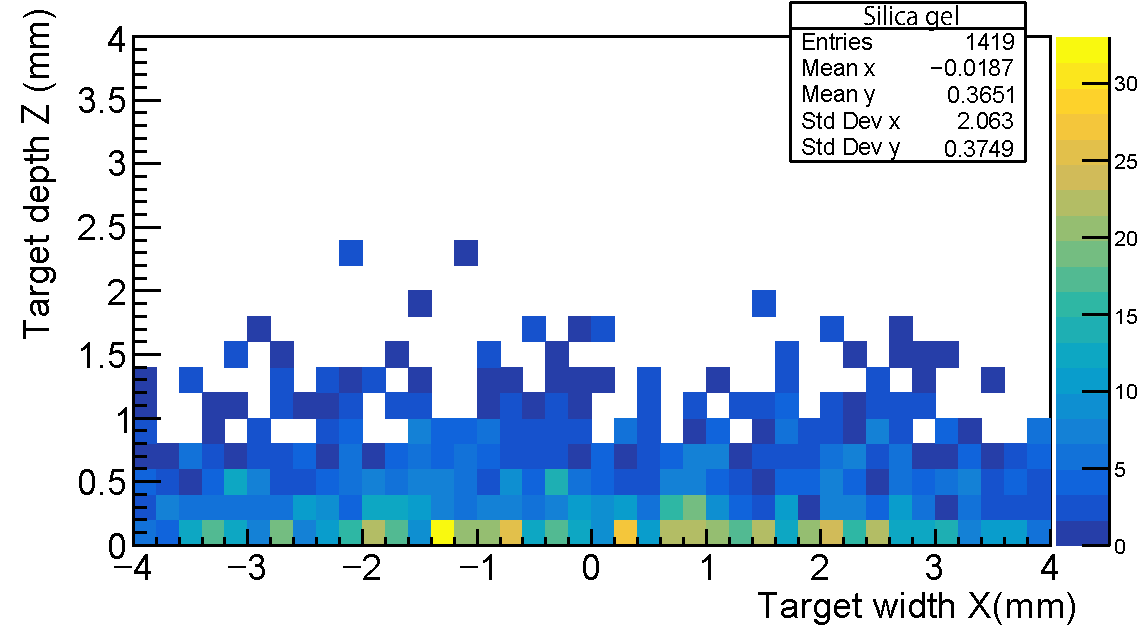
\includegraphics[width=10cm]{fig/test2bXY.pdf}
	\caption{陽電子停止位置X-Y方向}
	\label{test2bXY}
\end{figure}

\begin{figure}[htbp]
	\centering
		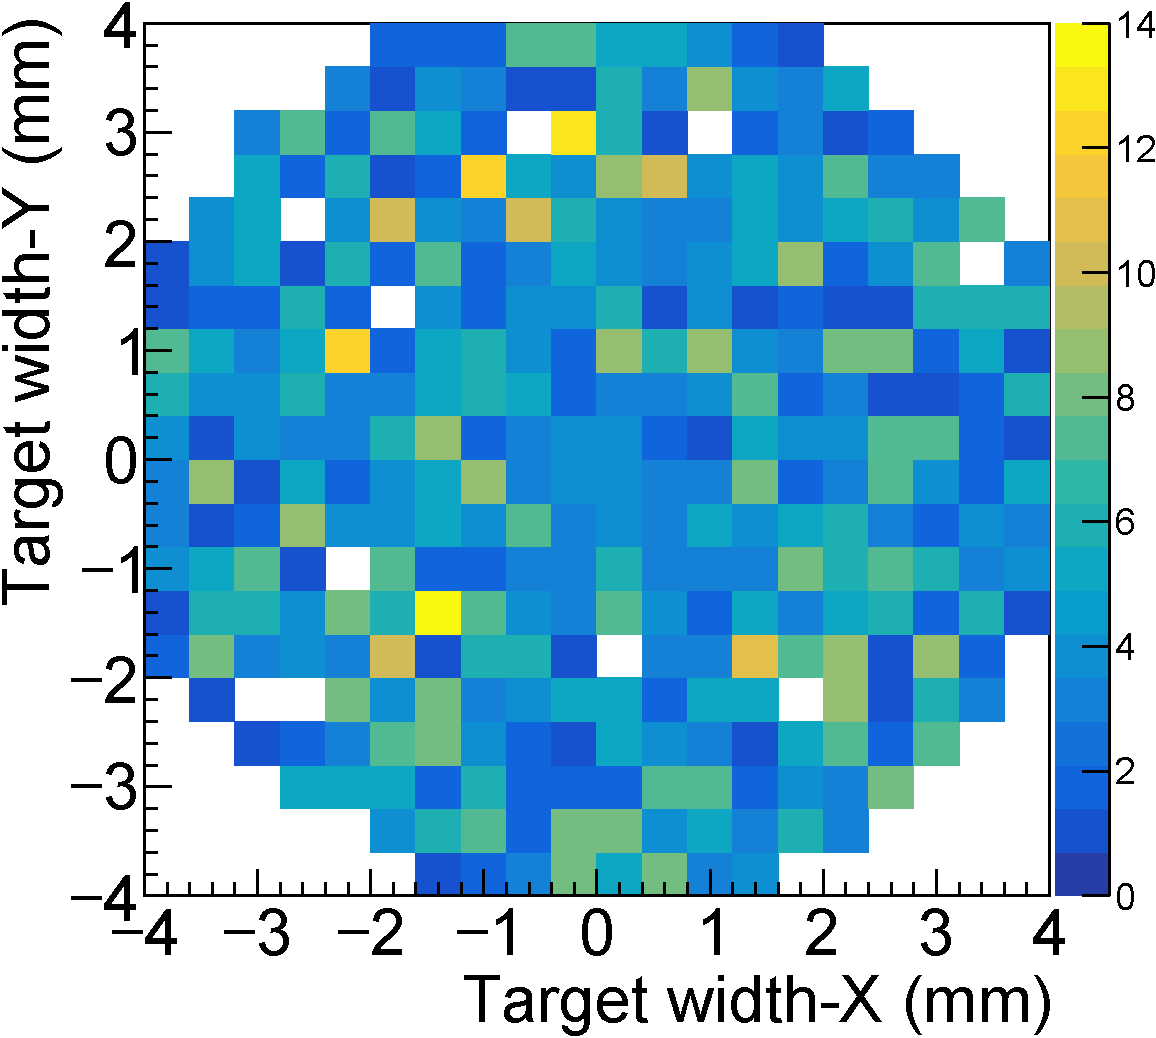
\includegraphics[width=7cm]{fig/test2bYZ.pdf}
	\caption{陽電子停止位置Y-Z方向}
	\label{test2bYZ}
\end{figure}

\subsection{考察}

図\ref{test2}は\ce{^{22}Na}の崩壊に対するエネルギースペクトルを示している.バックグラウンド事象が非常に多いが,プラスチックシンチレータを用いたトリガーを用いてアクシデンタル事象を除くバックグラウンドのほとんどを落とすことができると期待される.具体的なイベントレートとアクシデンタル由来のバックグラウンドレートの値については全てのシミュレーションを終えて第\ref{section_testall}節で検討する.また,エネルギーによるカットをかけられることが同時に期待される.

表\ref{table_test2}で,鉛コリメータを置くことでイベント数は7 \%程度になってしまうが,一方でバックグラウンド事象を1 \%近くまで落とすことができる.
本実験において,鉛コリメータが有用であるということが示された.

図\ref{test2bXY}から陽電子はシリカエアロゲル中で,平均して0.3 mmの深さで停止し,2 mm以下でほぼ全ての陽電子が停止する.
シリカエアロゲルケースは15 mmの深さで設計されており,陽電子の貫通に対して十分に深いと考えられる.
図\ref{test2bYZ}ではシンチレータの大きさに対してほぼ均等に陽電子が到達していることがわかる.
設計の直径8 mmは薄いシンチレータの強度に由来する最大の値であるためこれ以上大きくすることはできないが,シンチレータをこれ以上小さくする必要はないと言える.


\section{予想されるエネルギースペクトル}
\label{section_test3}

\subsection{ポジトロニウムの崩壊}

先だって行った2つのシミュレーションにより,我々の実験でのイベント頻度が概算された.最後に,この実験によって実際にどのような物理量が得られるべきか検討する.
公式にリリースされているGeant4にはポジトロニウムの様なエキゾチック原子の挙動は含まれておらず,前項でのシミュレーションでは陽電子はシリカゲル中で2$\gamma$崩壊していた.本項ではパラポジトロニウムとオルソポジトロニウムの崩壊を実装し,NaIシンチレータで検出する確率とエネルギースペクトルを推定する.また,オルソポジトロニウムの$3\gamma$崩壊を検討し第\ref{section_test2}節で行った評価に補正を加える.

実際にはスピン交換反応や,ピックオフ反応が起こり,実際に入射した陽電子がオルソポジトロニウムを形成し,$3\gamma$に崩壊する確率の理論的な予測は不可能であるため,$2\gamma$に崩壊する事象と$3\gamma$に崩壊する事象を同数シミュレーションを行う.

\subsection{結果}

図\ref{gamma2}はパラポジトロニウムに典型な$2\gamma$崩壊,図\ref{gamma3}はオルソポジトロニウムに典型な$3\gamma$崩壊の期待される実験スペクトルである.
装置の分解能は含まれていない.

\begin{figure}[htbp]
	\begin{tabular}{cc}

	\centering
		\begin{minipage}{0.5\hsize}
		\includegraphics[width=7cm]{fig/gamma2.pdf}
	\caption{観測される$2\gamma$崩壊のスペクトル}
	\label{gamma2}
		\end{minipage}&

		\begin{minipage}{0.5\hsize}
	\centering
		\includegraphics[width=7cm]{fig/gamma3.pdf}
	\caption{観測される$3\gamma$崩壊のスペクトル}
	\label{gamma3}
		\end{minipage}

		\end{tabular}
\end{figure}

\subsection{考察}
図\ref{gamma2}で示される2$\gamma$崩壊では電子と陽電子の質量に等しい511 keVの$\gamma$線が発生し,光電ピークとして現れている.
一方,図\ref{gamma3}で示される$3\gamma$崩壊では連続スペクトルが観測される.


\section{その他の物理量の概算}
\label{section_other}

\subsection{$3\gamma$崩壊事象と$2\gamma$崩壊事象との比の推定}
以上の各評価を統合して,実験レートとバックグラウンドレートを推定する.前述の様に$2\gamma$事象と$3\gamma$事象の比は理論で予測することはできない.オルソポジトロニウムとパラポジトロニウムの生成比は3:1であるが,オルソポジトロニウムはスピン交換反応をおこしパラポジトロニウムに変わってしまう.
また,ポジトロニウム中の陽電子が周囲の原子分子中の電子と対消滅するピックオフ消滅も起こる.
ピックオフ消滅を減らすため,シリカエアロゲルを真空状態に保つ工夫をしているが,無視することはできない.
したがって定量的な予測を行うことはできず昨年度の本研究室の卒業研究の結果などから$2\gamma$事象と$3\gamma$事象数が1:1であると見積もった.

\subsection{プラスチックシンチレータのトリガー効率}
陽電子,あるいは$\gamma$線がシンチレータでエネルギーを落とすことはMonte Carloシミュレーションで確かめることができる.
一方で,シンチレータの発光による光子が確実にPMTで検出されるかはわからない.
このトリガー効率を非常にラフではあるが10\%と見積もる.この効率については宮辺が議論した.

\subsection{2$\gamma$事象由来のバックグラウンド}
すくないということをいう予定.
詳細は実験データを元に第\ref{subsection_discussion}項で議論する.

\subsection{宇宙線由来のバックグラウンド}
すくないということをいう予定.

\subsection{自然放射線由来のバックグラウンド}
すくないということをいう予定.

\section{実験評価のまとめ}
\label{section_testall}

\subsection{実験レートとバックグラウンドの推定}
推定される実験でのイベントレートは図\ref{test1}から予測されるシリカゲルへの陽電子の到達確率,プラスチックシンチレータのトリガー効率,$3\gamma$事象の比,図\ref{gamma3}で予測される$\gamma$線がNaIシンチレータで検出される確率と,線源強度200 kBqの積として求められる.

\begin{equation}
	\frac{13,550}{10 \mathrm{M}} \times \frac{10}{100} \times \frac{1}{2} \times \frac{2,418,889}{10 \mathrm{M}} \times 200 \mathrm{ kBq} \sim 3.3 \mathrm{ Hz}
\end{equation}
ゆえにイベントレートは3.3 Hzと求められる.

図\ref{test2}からトリガーをかける前のバックグラウンド事象のレートを求めると,
\begin{equation}
	\frac{127,455}{100\mathrm{M}} \times 200 \mathrm{kBq} \sim 250 \mathrm{ Hz}
\end{equation}
ゆえに,トリガーをかけても落としきれないアクシデンタル事象のレートは,トリガーでゲートを1$\mu$s開くとして,
\begin{equation}
	( 1 \mu \mathrm{s} + 1 \mu \mathrm{s} ) \times  250 \mathrm{Hz} \times 3.3 \mathrm{Hz} \sim 1.7 \times 10^{-3} \mathrm{Hz}
\end{equation}
であり,目標としていたレート1 Hz, S/N比100のデザインをみたしていると言える.図\ref{test_all}はこのレートで1週間の測定を行った際に期待されるスペクトルである.

\begin{figure}[htbp]
	\centering
		\includegraphics[width=10cm]{fig/test_all.pdf}
	\caption{1週間の測定で期待されるスペクトル(若干修正予定)}
	\label{test_all}
\end{figure}

\subsection{議論}
\label{subsection_discussion}
現実の実験との比較について話す予定.
これ以前では実験前に考察したという体で,このセクションでは実験データ込みで装置分解能を含めたMonte Carloとの比較を行う.


